\section{Distribución de Probabilidad Discreta}
\subsection*{273}
Dada la variable aleatoria $X$ con distribución $\{ 1,\ldots ,n \}$. Calculamos lo siguiente
\begin{itemize}
	\item $\mathbf{E(X)}$ Por definición
		$$E(X) = \sum _{i=0} ^n x_i f(x_i) = \frac{1}{n} \underbrace{\sum _{i=0} ^n x_i}_{\frac{n(n+1)}{2}} = \frac{n+1}{2}.$$
	\item $\mathbf{E(X^2)}$ Por definición
		$$E(X^2) = \sum _{i=0} ^n x_i ^2 f(x_i) = \frac{1}{n} \underbrace{\sum _{i=0} ^n x_i ^2 x_i ^2}_{\frac{n(n+1)(2n+1)}{6}} = \frac{(n+1)(2n+1)}{6} .$$
	\item $\mathbf{V(X)}$ Por definición de varianza
		$$V(X) = E(X^2) - E(X)^2 = \frac{(n+1)(2n+1)}{6} - \frac{n+1}{2},$$
	simplificando con Mathematica (porque ya no estamos para estos trotes xD)
		$$V(X) = \frac{n^2 - 1}{12} .$$
\end{itemize}

\section{Distribución de Probabilidad de Bernoulli}
\subsection*{286}
Teniendo la varianza para la distribución de Bernoulli $V(X) = p(1-p)$, encontramos $p$ para maximizar $V(X)$,
	$$\dv{p} V(X) = 1-2p = 0 \quad \quad \Rightarrow \quad \quad \boxed{p=\frac{1}{2}}.$$
\section{Distribución de Probabilidad Binomial}
\subsection*{305}
Dados los datos $p = 0.9$ y $n = 20$, queremos obtener la probabilidad de no tener el ni el mínimo de éxito, es decir, $x = 18$, por ende queremos la probabilidad acumulada hasta $x = 17$. Utilizando la siguiente función de \textit{R}: \texttt{pbinom(17, size = 20, prob = 0.9)}. Con dicha función se tiene $P(X\leq 17) = \displaystyle\sum _{x=0} ^{17} \binom{20}{x} p^x (1-p)^{20-x} = 0.3230732.$


\section{Distribución de Probabilidad Geométrica}
\subsection*{311}
Dada la ecuación propuesta $E(X) = \sum_{x = 0} ^\infty (1 - F(x))$, reemplazando $F(x) = 1 - (1 - p)^{x + 1}$, entonces
	$$ E(X) = \sum _{x = 0} ^\infty (1 - p)^{x + 1} = \frac{1 - p}{1 - 1 + p} = \frac{1 - p}{p}. $$

\section{Distribución de Probabilidad Binomial Negativa}
\subsection*{331}
Dado que necesitamos $n$ lanzamientos y $r = 6$ éxitos; por ende, el número de fracasos $x = n - r$. Sustituyendo en la función de densidad de probabilidad
	$$\boxed{f(n - 6) = \binom{n - 1}{n - 6} \qty(\frac{1}{6})^6 \qty(\frac{5}{6})^{n - 6} .}$$

\section{Distribución de Probabilidad Hipergeométrica}
\subsection*{341}
Dados los datos, se tiene $N = 100$, $K = 90$, $n = 5$ y $x \in [2,n]$. Con esto, dado que queremos la probabilidad de que se realize la compra, calculamos
	$$1 - \sum _{x = 2} ^5 \frac{\binom{90}{x} \binom{10}{5 - x}}{\binom{100}{5}} = 0.9231433.$$
Para esto se utilizó \textit{R}. \\
{\tt
var1 <- 0 \\
for (i in 2:5)\{ \\
var1 <- var1 + dhyper(i,90,10,5) \\
\}
}

\section{Distribución de Probabilidad de Poisson}
\subsection*{343}
Encontrando el valor esperado $E(X)$
\begin{align*}
	E(X) &= \sum _x ^\infty x e^{-\lambda} \frac{\lambda ^x}{x!} \\
	&= \sum _x ^\infty e^{-\lambda} \frac{\lambda ^x}{(x - 1)!}
\end{align*}
\begin{align*}
	&= \lambda e^{-\lambda} \underbrace{\sum _x ^\infty \frac{\lambda ^{x - 1}}{(x - 1)!}}_{e^\lambda} \\
	&= \lambda .
\end{align*}

Ahora, encontrando la varianza $V(X) = E(X^2) - E(X)^2$, encontramos la esperanza de $X^2$
	\begin{align*}
		E(X^2) &= \sum _x x^2 e^{-\lambda} \frac{\lambda ^x}{x!} \\
		&= \sum _x \lambda xe^{-\lambda} \frac{\lambda ^{x - 1}}{(x - 1)!} \\
		&= \lambda e^{-\lambda} \sum _j (j + 1) \frac{\lambda ^j}{j!} \\
		&= \lambda e^{-\lambda} \qty[\underbrace{\sum _j j\frac{\lambda ^j}{j!}}_{\lambda e^\lambda} + \underbrace{\sum _j \frac{\lambda ^j}{j!}}_{e^\lambda}] \\
		&= \lambda ^2 + \lambda ,
	\end{align*}

entonces
\begin{align*}
	V(X) &= \lambda ^2 + \lambda - \lambda ^2 \\
	&= \lambda .
\end{align*}



\section{Distribución de Probabilidad Uniforme Continua}
\subsection*{357}

\begin{enumerate}[a)]
	\item Entontrando $E(X)$, se tiene que $f(x) = \frac{1}{b-a}$, entonces
		$$E(X) = \int _a ^b \frac{x}{b-a} \dd{x} = \frac{1}{b-a} \frac{b^2 - a^2}{2} = \frac{a+b}{2}.$$
	\item Encontrando $E(X^2)$, entonces, realizando la integral
		$$\int _a ^b \frac{x^2}{b-a} \dd{x} = \frac{1}{b-a} \frac{b^3 - a^3}{3} = \frac{b^2 + ab + a^2}{3}.$$
	\item Encontrando la varianza,
		$$Var(X) = E(X^2) - E(X)^2 = \frac{a^2 + ab + b^2}{3} - \frac{(a + b)^2}{4} = \frac{a^2 + b^2}{12} - \frac{ab}{6} = \frac{(a - b)^2}{12}.$$
\end{enumerate}


\section{Distribución de Probabilidad Exponencial}
\subsection*{375}
Encontramos el enésimo momento, $E(X^n)$, realizando la integral
	$$E(X^n) = \lambda \int _0 ^\infty x^n e^{-\lambda x} \dd{x},$$
realizando el cambio de variable $\lambda x = t$, se tiene
	$$\int _0 ^\infty \qty(\frac{t}{\lambda})^n e^{-t} \dd{t} = \frac{1}{\lambda ^n} \int _0 ^\infty t^n e^{-t} \dd{t},$$
la cual es exactamente a la función Gamma valuada en $n+1$, $\Gamma (n+1) = n!$, por lo tanto
	$$E(X^n) = \frac{\Gamma (n+1)}{\lambda ^n} = \frac{n!}{\lambda ^n}.$$


\section{Distribución Gamma}
\subsection*{386}
Por definición de esperanza, se tiene
	$$E(X) = \int _0 ^\infty x \frac{(\lambda x)^{\alpha - 1}}{\Gamma (\alpha)} \lambda e^{-\lambda x} \dd{x} = \frac{1}{\Gamma (\alpha)} \underbrace{\int _0 ^\infty \frac{u}{\lambda} u^{\alpha - 1} e^{-u} \dd{u}}_{\frac{1}{\lambda} \Gamma (\alpha + 1)},$$
	entonces, por propiedades de la función gamma, $\Gamma (\alpha + 1) = \alpha \Gamma (\alpha)$; por lo que,
	$$E(X) = \frac{\alpha}{\lambda}.$$
Para el resto de calculos se utiliza exactamente la misma idea, de modo que
	$$E(X^2) = \int _0 ^\infty x^2 \frac{(\lambda x)^{\alpha - 1}}{\Gamma (\alpha)} \lambda e^{-\lambda x} \dd{x} = \frac{1}{\Gamma (\alpha)} \underbrace{\int _0 ^\infty \frac{1}{\lambda ^2} u^{\alpha + 1} e^{-u} \dd{u}}_{\frac{1}{\lambda ^2} \Gamma (\alpha + 2)},$$
siguiendo la recursividad de la función gamma, se tiene
	$$E(X^2) = \frac{\alpha (\alpha + 1)}{\lambda ^2}.$$
Lo mismo para $E(X^3)$,
	$$E(X^2) = \int _0 ^\infty x^3 \frac{(\lambda x)^{\alpha - 1}}{\Gamma (\alpha)} \lambda e^{-\lambda x} \dd{x} = \frac{1}{\Gamma (\alpha)} \underbrace{\int _0 ^\infty \frac{1}{\lambda ^3} u^{\alpha + 2} e^{-u} \dd{u}}_{\frac{1}{\lambda ^3} \Gamma (\alpha + 3)},$$
	entonces 
	$$E(X^3) = \frac{(\alpha + 2)(\alpha + 1)\alpha}{\lambda ^3}.$$
Encontrando la varianza $\text{Var} (X) = E(X^2) - E(X)^2$
	$$\text{Var} (X) = \frac{\alpha (\alpha + 1)}{\lambda ^2} - \qty(\frac{\alpha}{\lambda})^2 = \frac{\alpha}{\lambda ^2}.$$


\section{Distribución Beta}
\subsection*{398}
Calculando $E(X^n)$
	$$E(X^n) = \frac{1}{B(a,b)} \int _0 ^1 x^n x^{a - 1} (1 - x)^{b - 1} \dd{x} = \frac{1}{B(a,b)} \underbrace{\int _0 ^1 x^{a + n - 1} (1 - x)^{b - 1} \dd{x}}_{B(a + n,b)} = \frac{B(a + n,b)}{B(a,b)}.$$
	
\section{Distribución Weibull}
\subsection*{405}
Realizando la sustitución $u = (\lambda x)^\alpha$, entonces calculando 
	$$E(X^n) = \int _0 ^\infty x^n \underbrace{(\alpha \lambda) (\lambda x)^{\alpha -1} e^{-(\lambda x)^\alpha}}_{f(x)} \dd{x} = \int _0 ^\infty \frac{u^{\flatfrac{n}{\alpha}}}{\lambda ^n} e^{-u} \dd{u} = \frac{\Gamma(1 + \flatfrac{n}{\alpha})}{\lambda ^n}.$$


\section{Distribución Normal}
\subsection*{412}
Por definición la mediana es $\mu$. Para la moda, derivamos e igualamos a cero
	$$\dv{f(x)}{x} = - \frac{e^{-\frac{(x - \mu)^2}{2\sigma ^2}} (x - \mu)}{\sqrt{2\pi} \sigma ^3} = 0,$$
entonces
	$$ x_{\text{moda}} = \mu. $$


\section{Distribución Ji-Cuadrada}
\subsection*{430}
Se plantea la integral y la sustitución $u = \flatfrac{x}{2}$, entonces
	$$ E(X^m) = \frac{1}{2^{\flatfrac{n}{2}} \Gamma (\flatfrac{n}{2})} \int _0 ^\infty x^{\frac{n}{2} + m - 1} e^{-\flatfrac{x}{2}} \dd{x} = \frac{2^{\frac{n}{2} + m - 1}}{2^{\frac{n}{2} - 1} \Gamma (\flatfrac{n}{2})} \underbrace{\int _0 ^\infty u^{\frac{n}{2} + m - 1} e^{-u} \dd{u}}_{\Gamma (\flatfrac{n}{2} + m)} = \frac{2^m}{\Gamma (\flatfrac{n}{2})} \Gamma (\flatfrac{n}{2} + m). $$


\section{Distribución $t$}
\subsection*{438}
Para esto, ploteamos la función de distribución para distintos $n$ en el mismo intervalo en \textit{mathematica}
\begin{figure}[H]
	\centering
	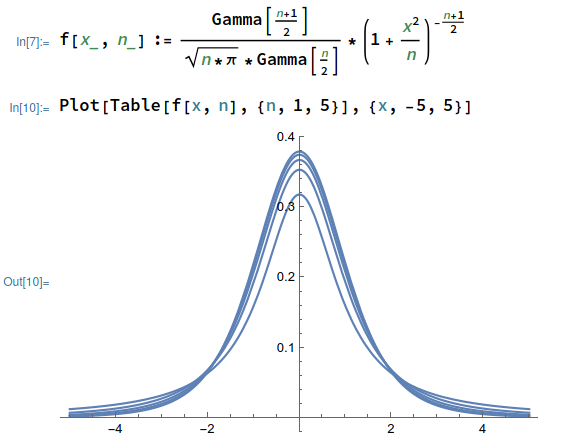
\includegraphics[scale=0.5]{img/t.png}
	\caption{Función de distribución $f(x) = \frac{\Gamma \qty(\frac{n+1}{2})}{\sqrt{n\pi} \, \Gamma \qty(\flatfrac{n}{2})} \qty(1+\frac{x^2}{n})^{-\frac{n+1}{2}}$, para $n = 1,2,3,4,5$.}
\end{figure}
Con lo que es claro que la moda y la mediana coinciden en $0$.


\section{Distribución F}
\subsection*{443}
Tomando la maximizando la función de distribución, se tiene que la derivada igualada a cero es (con ayuda de \textit{mathematica})
	$$ -\frac{\left(\frac{a}{b}\right)^{a/2} x^{\frac{a}{2}-2} \left(\frac{a x}{b}+1\right)^{-\frac{a}{2}-\frac{b}{2}} (a b x-a b+2 a x+2 b) \Gamma \left(\frac{a+b}{2}\right)}{2 \Gamma \left(\frac{a}{2}\right) \Gamma \left(\frac{b}{2}\right) (a x+b)}=0, $$
entonces, una de las soluciones es $(a b x-a b+2 a x+2 b)=0$; por lo tanto
	$$ (a b x-a b+2 a x+2 b) = 0, \quad \quad \quad \Rightarrow \quad \quad \quad x = \frac{b(a - 2)}{a(b + 2)}. $$





















%%%